\section{Extensions}
\label{kvdirect:sec:extensions}

\subsection{CPU-based Scatter-Gather DMA}

PCIe has 29\% TLP header and padding overhead for 64B DMA operations (\S\ref{kvdirect:sec:challenge}) and the DMA engine may not have enough parallelism to saturate the PCIe bandwidth-delay product with small TLPs (\S\ref{kvdirect:sec:implementation}).
Larger DMA operations with up to 256-byte TLP payload is supported by the PCIe root complex in our system. In this case, the TLP head and padding overhead is only 9\%, and the DMA engine has enough parallelism (64) to saturate the PCIe link with 27 in-flight DMA reads.
To batch the DMA operations on PCIe link, we can leverage the CPU to perform scatter-gather (Figure~\ref{kvdirect:fig:sg-arch}).
First, the NIC DMAs addresses to a request queue in host memory. The host CPU polls the request queue, performs random memory access, put the data in response queue and writes MMIO doorbell to the NIC. The NIC then fetches the data from response queue via DMA.

\begin{figure}[t]
\centering
\subfloat[Read.\label{kvdirect:fig:sge-read}]
{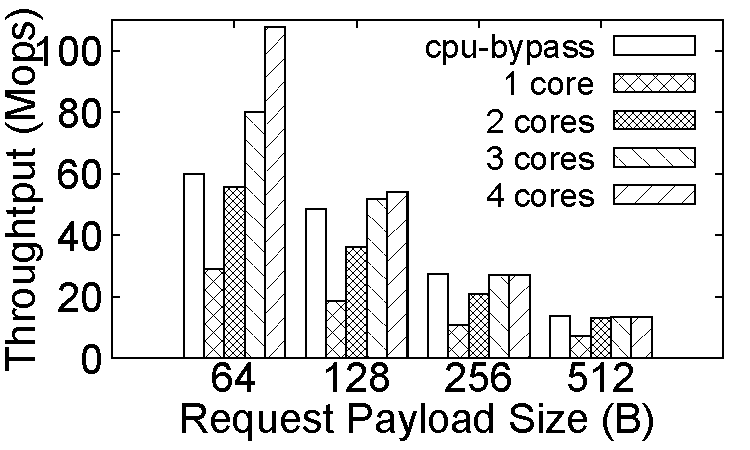
\includegraphics[width=.5\textwidth,page=1]{sg-read.pdf}}
\subfloat[Write.\label{kvdirect:fig:sge-write}]
{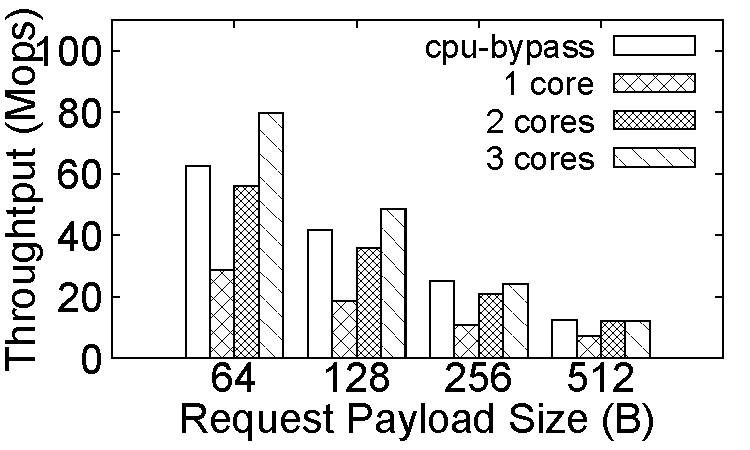
\includegraphics[width=.5\textwidth,page=1]{sg-write.pdf}}
\caption{Scatter-gather performance.}
\label{kvdirect:fig:scatter-gather}

\end{figure}

Figure~\ref{kvdirect:fig:scatter-gather} shows that CPU-based scatter-gather DMA has up to 79\% throughput improvement compared to the CPU-bypassing approach.
In addition to the CPU overhead, the primary drawback of CPU-based scatter-gather is the additional latency.
To save MMIOs from the CPU to the NIC, we batch 256 DMA operations per doorbell, which requires 10~$\mu$s to complete.
The overall latency for the NIC to access host memory using CPU-based scatter-gather is \approx20~$\mu$s, almost 20x higher than direct DMA.

\subsection{Multiple NICs per Server}
\label{kvdirect:sec:multi-nic}

\begin{figure}[t]
\begin{minipage}[t]{0.5\textwidth}
\centering
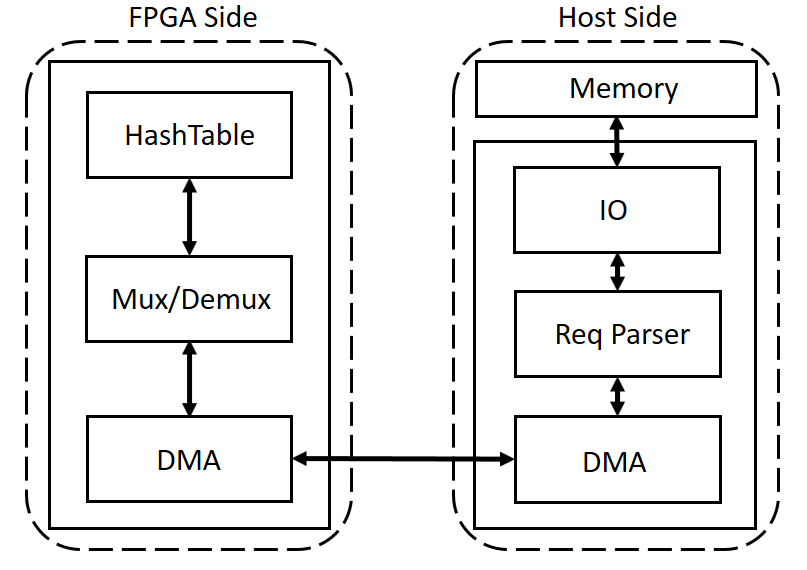
\includegraphics[width=1\textwidth,page=1]{scatter_gather.PNG}
\caption{Scatter-gather architecture.}
\label{kvdirect:fig:sg-arch}
\end{minipage}
\begin{minipage}[t]{0.5\textwidth}
\centering
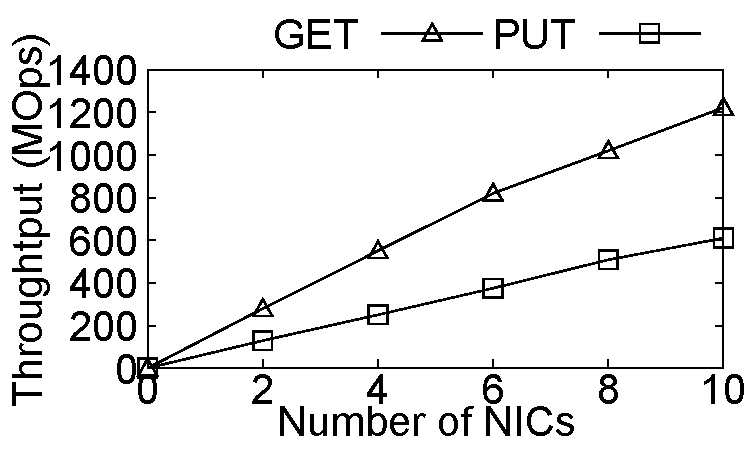
\includegraphics[width=1\textwidth,page=1]{multi_nic.pdf}
\caption{Performance of multiple NICs per server.}
\label{kvdirect:fig:multiple-nics}
\end{minipage}

\end{figure}

%The primary use case for KV-Direct is to enable remote direct key-value access without CPU overhead on the server. 
In some cases, it may be desirable to build a dedicated key-value store with maximal throughput per server.
Through simulation, \cite{li2016full} showed the possibility of achieving a billion KV op/s in a single server with four (currently unavailable) 60-core CPUs.
As shown in Table~\ref{kvdirect:tab:kvs-compare}, with 10 KV-Direct NICs on a server, the one billion KV op/s performance is readily achievable with a commodity server.
The server consumes 357 watts power (measured on the wall) to achieve 1.22~Gop/s GET or 0.61~Gop/s PUT.

In order to saturate the 80 PCIe Gen3 lanes of two Xeon E5 CPUs, we replace the motherboard of the benchmarked server (Sec.~\ref{kvdirect:sec:eval}) with a SuperMicro X9DRX+-F motherboard with 10 PCIe Gen3 x8 slots.
We use PCIe x16 to x8 converters to connect 10 programmable NICs on each of the slots, and only one PCIe Gen3 x8 link is enabled on each NIC, so the throughput per NIC is lower than Figure~\ref{kvdirect:fig:ycsb-tput}.
Each NIC owns an exclusive memory region in host memory and serves a disjoint partition of keys.
Multiple NICs suffer the same load imbalance problem as a multi-core KVS implementation.
Fortunately, for a small number of partitions (\textit{e.g.} 10), the load imbalance is not significant~\cite{lim2014mica,li2016full}. Under YCSB long-tail workload, the highest-loaded NIC has 1.5x load of the average, and the added load from extremely popular keys is served by the out-of-order execution engine (Sec.~\ref{kvdirect:sec:ooo}).
%In comparison, to achieve matching performance with 240 CPU cores, the load of the hottest core will be 10x of the average.
Figure~\ref{kvdirect:fig:multiple-nics} shows that KV-Direct throughput scales almost linearly with the number of NICs on a server.



\subsection{Discussion}
\label{kvdirect:sec:discussion}

\subsubsection{NIC hardware with different capacity.}
\label{kvdirect:sec:different-nic}

The goal of KV-Direct is to leverage existing hardware in data centers to offload an important workload (KV access), instead of designing a special hardware to achieve maximal KVS performance. We use programmable NICs, which usually contain limited amount of DRAM for buffering and connection-state tracking. Large DRAMs are expensive in both die size and power consumption.
%Our Hynix DDR3 SDRAM takes 35 $mm^2$ die size per 4 Gb, and will occupy 4480 $mm^2$ for 64 GB, much larger than the 1600 $mm^2$ die size of our Stratix V FPGA. In terms of power consumption, 64 GB of on-board DRAM will consume 56 watts (assuming 0.878 watt/GB in~\cite{blott2015scaling}), much larger than TDP of our entire FPGA board (30 watts).

\begin{table}[t]
\centering
\scalebox{0.85}{
\begin{tabular}{|l|r|r|r|r|r|r|}
\hline
     & 1/1024 & 1/256 & 1/64 & 1/16 & 1/4 & 1 \\
\hline
1/2  & 0.366 & 0.358 & 0.350 & 0.342 & 0.335 & 0.327 \\
\hline
1    & 0.583 & 0.562 & 0.543 & 0.525 & 0.508 & 0.492 \\
\hline
2    & 0.830 & 0.789 & 0.752 & 0.718 & 0.687 & 0.658 \\
\hline
4    & 1     & 0.991 & 0.933 & 0.881 & 0.835 & 0.793 \\
\hline
8    & 1     & 1     & 1     & 0.995 & 0.937 & 0.885 \\
\hline
\end{tabular}
}
\caption{Optimal load dispatch ratio for long-tail workload under different NIC DRAM/PCIe throughput ratio (vertical) and NIC/host memory size ratio (horizontal).}
\label{kvdirect:tab:optimal-load-dispatch}

\end{table}

\begin{table}[t]
\centering
\scalebox{0.85}{
\begin{tabular}{|l|r|r|r|r|r|r|}
\hline
    & 1/1024 & 1/256 & 1/64 & 1/16 & 1/4 & 1 \\
\hline
1/2 & 1.36	& 1.39	& 1.40	& 1.37	& 1.19	& 1.02 \\ 
\hline
1	& 1.71	& 1.77	& 1.81	& 1.79	& 1.57	& 1.01 \\
\hline
2	& 2.40	& 2.52	& 2.62	& 2.62	& 2.33	& 1.52 \\
\hline
4	& 3.99	& 4.02	& 4.22	& 4.27	& 3.83	& 2.52 \\
\hline
8	& 7.99	& 7.97	& 7.87	& 7.56	& 6.83	& 4.52 \\
\hline
\end{tabular}
}
\caption{Relative throughput of load dispatch compared to simple partitioning. Column titles are same as Table~\ref{kvdirect:tab:optimal-load-dispatch}.}
\label{kvdirect:tab:optimal-load-dispatch-throughput}

\end{table}


Even if future NICs have faster or larger on-board memory, under long-tail workload, our load dispatch design (Sec.~\ref{kvdirect:sec:dram-cache}) still shows performance gain over the simple design of partitioning the keys uniformly according to NIC and host memory capacity.
Table~\ref{kvdirect:tab:optimal-load-dispatch} shows the optimal load dispatch ratio for long-tail workload with a corpus of 1 billion keys, under different ratio of NIC DRAM and PCIe throughput and different ratio of NIC and host memory size.
If the NIC has faster DRAM, more load will be dispatched to the NIC. A load dispatch ratio of 1 means the NIC memory behaves exactly like a cache of host memory.
If the NIC has larger DRAM, a slightly less portion of load will be dispatched to the NIC.
As shown in Table~\ref{kvdirect:tab:optimal-load-dispatch-throughput}, even when the size of NIC DRAM is a tiny fraction of host memory, the throughput gain is significant.

The out-of-order execution engine (Sec.~\ref{kvdirect:sec:ooo}) can be applied to all kinds of applications in need of latency hiding, and we hope future RDMA NICs to support that for atomics.

In 40~Gbps networks, network bandwidth bounds non-batched KV throughput, so we use client-side batching (Sec.\ref{kvdirect:sec:implementation}). With higher network bandwidth, batch size can be reduced, thus reducing latency. In a 200~Gbps network, a KV-Direct NIC could achieve 180~Mop/s without batching.

KV-Direct leverages widely-deployed programmable NICs with FPGAs~\cite{putnam2014reconfigurable,caulfield2016cloud}. FlexNIC~\cite{kaufmann2015flexnic,kaufmann2016krishnamurthy} is another promising architecture for programmable NICs with Reconfigurable Match-action Tables (RMT)~\cite{bosshart2013forwarding}.
NetCache~\cite{netcache-sosp17} implements a KV cache in RMT-based programmable switches, showing potential for building KV-Direct in an RMT-based NIC.

\subsubsection{Implications for real-world applications.}

Back-of-the-envelope calculations show potential performance gains when KV-Direct is applied in end-to-end applications. In PageRank~\cite{page1999pagerank}, because each edge traversal can be implemented with one KV operation, KV-Direct supports 1.22G TEPS on a server with 10 programmable NICs. In comparison, GRAM~\cite{wu2015g} supports 250M TEPS per server, bound by interleaved computation and random memory access.

KV-Direct supports user-defined functions and vector operations (Table~\ref{kvdirect:tab:kv-operations}) that can further optimize PageRank by offloading client computation to hardware. Similar arguments hold for parameter server~\cite{li2014scaling}. We expect future work to leverage hardware-accelerated key-value stores to improve distributed application performance.
